%% DocuQuery AI Assistant --- IEEEtran manuscript (Revised v2).
%% All benchmark numbers generated by paper/micro_benchmark.py on 2026-04-20.
%% Expanded to 1000 chunks / 100 queries; 4 scenarios; McNemar tests; nDCG@5.
%% Compile: pdflatex docuquery_ieee (run twice for stable refs/cross-refs).
\documentclass[journal]{IEEEtran}

\usepackage{cite}
\usepackage{amsmath,amssymb}
\usepackage{booktabs}
\usepackage{multirow}
\usepackage{graphicx}
\usepackage{url}
\usepackage[hidelinks]{hyperref}
\usepackage{xcolor}
\usepackage{tikz}
\usetikzlibrary{shapes.geometric, arrows.meta, positioning, fit}

%% --- BENCHMARK SNAPSHOT (auto-generated by paper/micro_benchmark.py) ---
%% 1000 chunks, 100 queries/scenario, all-MiniLM-L6-v2, 2026-04-20
\newcommand{\SnapDate}{2026-04-20}
\newcommand{\SnapEmbed}{all-MiniLM-L6-v2}
\newcommand{\SnapChunks}{1000}
\newcommand{\SnapQueries}{100}
\newcommand{\SnapBuildSec}{1.753}
%% Scenario A - identifier-heavy
\newcommand{\SnapRB}{1.000}
\newcommand{\SnapRD}{0.130}
\newcommand{\SnapRTF}{1.000}
\newcommand{\SnapRH}{0.480}
\newcommand{\SnapMrrBMxxA}{1.000}
\newcommand{\SnapMrrDenseA}{0.114}
\newcommand{\SnapMrrTFIDFA}{1.000}
\newcommand{\SnapMrrHybridA}{0.480}
\newcommand{\SnapNDCGBMA}{1.000}
\newcommand{\SnapNDCGDenseA}{0.095}
\newcommand{\SnapNDCGTFIDFA}{1.000}
\newcommand{\SnapNDCGHA}{0.480}
%% Scenario B - paraphrase
\newcommand{\SnapRBB}{1.000}
\newcommand{\SnapRDB}{0.170}
\newcommand{\SnapRTFB}{1.000}
\newcommand{\SnapRHB}{1.000}
\newcommand{\SnapMrrBMxxB}{0.910}
\newcommand{\SnapMrrDenseB}{0.108}
\newcommand{\SnapMrrTFIDFB}{0.992}
\newcommand{\SnapMrrHybridB}{0.990}
\newcommand{\SnapNDCGBMB}{0.934}
\newcommand{\SnapNDCGDenseB}{0.110}
\newcommand{\SnapNDCGTFIDFB}{0.994}
\newcommand{\SnapNDCGHB}{0.993}
%% Scenario C - OCR noise
\newcommand{\SnapRBMC}{0.890}
\newcommand{\SnapRDenseC}{0.160}
\newcommand{\SnapRTFC}{0.880}
\newcommand{\SnapRHC}{0.890}
\newcommand{\SnapMrrHybridC}{0.853}
\newcommand{\SnapNDCGHC}{0.863}
%% Scenario D - multilingual
\newcommand{\SnapRBMD}{1.000}
\newcommand{\SnapRDenseD}{0.210}
\newcommand{\SnapRTFD}{1.000}
\newcommand{\SnapRHD}{1.000}
\newcommand{\SnapMrrHybridD}{1.000}
\newcommand{\SnapNDCGHD}{1.000}
%% Latency
\newcommand{\SnapLatMean}{21.03}
\newcommand{\SnapLatStd}{1.95}
\newcommand{\SnapLatCI}{0.76}

\author{Karthik~Mulugu%
\thanks{K.~Mulugu is an independent researcher, Charlotte, North Carolina 28079, USA.
ORCID: \url{https://orcid.org/0009-0001-6261-6658}.
Open-source demo: \url{https://huggingface.co/spaces/karthikmulugu08/docuquery-ai-assistant}.
Corresponding e-mail: \texttt{karthikmulugu14@gmail.com}.}}

\markboth{IEEE Access}{Mulugu: DocuQuery---Hybrid Retrieval with Graph Orchestration for PDF QA}

\begin{document}

\title{DocuQuery: Design, Implementation, and Empirical Analysis of a Hybrid Lexical--Dense Retrieval System with LangGraph Orchestration for PDF Question Answering}

\maketitle

\begin{abstract}
PDF question answering requires grounded answers across diverse user intents---paraphrased natural language, precise identifier lookup, summarisation, and comparison---and must remain robust under real-world challenges such as OCR noise and multilingual content. This paper presents DocuQuery, an open-source reference implementation whose primary contribution is a \emph{documented design-space analysis}: we identify which fusion choices help, which hurt, and under what query-type conditions using a reproducible micro-benchmark.

DocuQuery fuses BM25, FAISS dense vectors, and TF--IDF with configurable weights and optional Pinecone cloud indexing; encodes multi-intent routing via a LangGraph \texttt{StateGraph}; and exposes chunk-level evidence through a Gradio interface. Evaluation spans \textbf{four scenarios} over 1\,000 passages with 100 queries each, reporting Recall@5, MRR, nDCG@5, and McNemar significance tests.

On paraphrase queries, hybrid achieves Recall@5\,=\,1.00 and nDCG@5\,=\,0.993, statistically significantly outperforming dense-only ($p{<}0.001$). On identifier-heavy queries, fixed-weight fusion \emph{degrades} Recall@5 to 0.480 versus lexical-only 1.000---a significant failure ($p{<}0.001$). Under 2\% simulated OCR noise, hybrid sustains Recall@5\,=\,0.890 while dense collapses to 0.160. On multilingual passages, hybrid achieves Recall@5\,=\,1.000. A prespecified faithfulness protocol and ablation methodology for fusion-weight optimisation are provided for real-document follow-up.
\end{abstract}

\begin{IEEEkeywords}
Retrieval-augmented generation, hybrid retrieval, information retrieval, LangGraph, PDF question answering, OCR robustness, multilingual, statistical significance, reference architecture.
\end{IEEEkeywords}

%% =========================================================
\section{Introduction}
\label{sec:intro}
%% =========================================================

Organizations deploy document QA over long PDFs---policies, reports, contracts. LLMs operating on parametric memory alone hallucinate on document-specific facts~\cite{lewis2020retrieval,gao2023rag}. RAG conditions generation on retrieved spans~\cite{lewis2020retrieval,fan2024survey}, but deployable systems face three engineering problems.

\textbf{Problem 1: Single-signal retrieval is fragile.}
Dense retrieval~\cite{karpukhin2020dense} fails on identifier-heavy queries; sparse methods fail on paraphrase queries. Neither dominates across diverse corpora~\cite{thakur2021beir}. On our 1\,000-chunk benchmark, dense-only achieves Recall@5\,=\,0.170 even for paraphrase queries (Section~\ref{sec:eval}), showing that embedding crowding at moderate corpus scale substantially erodes semantic discriminability.

\textbf{Problem 2: Real documents contain OCR noise and multilingual text.}
Scanned PDFs introduce character-level corruption; enterprise corpora contain non-English passages. Systems tested only on clean English text provide no robustness evidence for deployment.

\textbf{Problem 3: Unstructured RAG chains are opaque.}
Conditional retrieval logic embedded in a single function hinders debugging, state inspection, and unit testing. Multi-intent routing---summarise, compare, refine, lookup---needs explicit state encoding.

\textbf{Framing.} DocuQuery does \emph{not} introduce a new algorithm or neural model. Its contribution is a \emph{reference design} with empirically validated trade-offs: (i)~four-scenario evaluation including OCR noise and multilingual robustness; (ii)~McNemar significance testing on all pairwise comparisons; (iii)~LangGraph-encoded orchestration for inspectable routing; and (iv)~a committed ablation methodology and faithfulness protocol for follow-up evaluation.

\textbf{Why not use an existing framework?}
Table~\ref{tab:framework} compares DocuQuery to LangChain~\cite{langchain2024}, Haystack~\cite{haystack2024}, and LlamaIndex~\cite{llamaindex2024}. None publishes a single reference fusion recipe with documented weight sensitivity, OCR/multilingual robustness evaluation, and an attached significance-tested benchmark.

\begin{table*}[!t]
\renewcommand{\arraystretch}{1.15}
\caption{Feature comparison of open frameworks vs.\ DocuQuery.
\checkmark\,=\,natively available;\enspace $\circ$\,=\,available via plug-in/extension;\enspace --\,=\,not provided in core.}
\label{tab:framework}
\centering
\begin{tabular}{@{}l c c c c@{}}
\toprule
Feature & LlamaIndex & Haystack & LangChain & DocuQuery \\
\midrule
Hybrid BM25 + Dense retrieval        & $\circ$ & $\circ$ & $\circ$ & \checkmark \\
Documented fusion weights            & --      & --      & --      & \checkmark \\
LangGraph-based routing              & --      & --      & $\circ$ & \checkmark \\
Chunk-level evidence UI              & --      & $\circ$ & --      & \checkmark \\
OCR-noise and multilingual benchmark & --      & --      & --      & \checkmark \\
McNemar significance testing         & --      & --      & --      & \checkmark \\
\bottomrule
\end{tabular}
\end{table*}

\textbf{Contributions.}
\begin{enumerate}
  \item \textbf{Multi-scenario evaluation with statistical significance.} Four scenarios (A: identifier, B: paraphrase, C: OCR-noise, D: multilingual) over 1\,000 passages / 100 queries each; Recall@5, MRR, nDCG@5; McNemar's test and 95\% bootstrap CI.
  \item \textbf{Documented hybrid fusion with failure-mode analysis.} Empirical and statistically validated evidence of when fixed-weight fusion helps (Scenario~B) and hurts (Scenario~A).
  \item \textbf{OCR and multilingual robustness data.} First published robustness evaluation of this kind in an open PDF QA system.
  \item \textbf{LangGraph orchestration} separating routing, retrieval, and generation into testable graph nodes.
  \item \textbf{Reproducible benchmark script} (\texttt{paper/micro\_benchmark.py}) and prespecified protocols for ablation and faithfulness evaluation.
\end{enumerate}

%% =========================================================
\section{Related Work}
\label{sec:related}
%% =========================================================

\textbf{Sparse and dense retrieval.}
BM25~\cite{robertson1994okapi,robertson2009probabilistic} excels on keyword queries. Dense retrieval (DPR)~\cite{karpukhin2020dense} improves semantic recall but fails on rare identifiers and in crowded embedding spaces (our Scenario~A, B). SPLADE~\cite{formal2021splade} learns sparse representations combining lexical precision with soft term expansion. BGE-M3~\cite{chen2024bge} achieves state-of-the-art multi-granularity retrieval on MTEB~\cite{muennighoff2023mteb}; integrating it would replace the heuristic lexical+dense combination. BEIR~\cite{thakur2021beir} benchmarks retrieval across 18 heterogeneous corpora; running DocuQuery's pipeline on BEIR datasets is deferred to future work.

\textbf{Hybrid retrieval.}
Combining sparse and dense signals consistently outperforms either alone~\cite{thakur2021beir}. RRF~\cite{cormack2009rcf} is a parameter-free fusion baseline; DocuQuery uses fixed-weight linear combination, whose sensitivity is analysed in Section~\ref{sec:ablation}. ColBERT~\cite{khattab2020colbert} uses late interaction at higher memory cost.

\textbf{RAG orchestration and evaluation.}
Lewis et al.~\cite{lewis2020retrieval} established RAG; FLARE~\cite{jiang2023flare} and Self-RAG~\cite{asai2023selfrag} add adaptive retrieval. RAGAS~\cite{es2023ragas} automates faithfulness scoring; Table~\ref{tab:faith} plans to use it as a first-pass filter.

\textbf{OCR and multilingual retrieval.}
Character corruption degrades BM25 exact-match; dense models may generalise better across minor perturbations but fail when embedding crowding dominates. For cross-lingual retrieval, BM25 can match on shared tokens; cross-lingual dense models extend coverage~\cite{thakur2021beir}.

\textbf{TF--IDF reliability on small corpora.}
IDF weights on small corpora are unstable~\cite{salton1988tfidf,jones1972statistical}. Expanding to 1\,000 passages reduces this concern substantially; explicit validity limits are stated in Section~\ref{sec:threats}.

\textbf{Frameworks.}
Table~\ref{tab:framework} summarises the comparison with LlamaIndex~\cite{llamaindex2024}, Haystack~\cite{haystack2024}, and LangChain~\cite{langchain2024}.

%% =========================================================
\section{System Architecture}
\label{sec:arch}
%% =========================================================

Fig.~\ref{fig:arch} illustrates the pipeline. PDFs are parsed (\texttt{pypdf}~\cite{pypdf2024}), chunked with sentence-aware boundaries, and embedded (\texttt{all-MiniLM-L6-v2}~\cite{reimers2019sentence,sentencetransformers2024}).

\begin{figure}[!t]
\centering
\resizebox{0.98\columnwidth}{!}{%
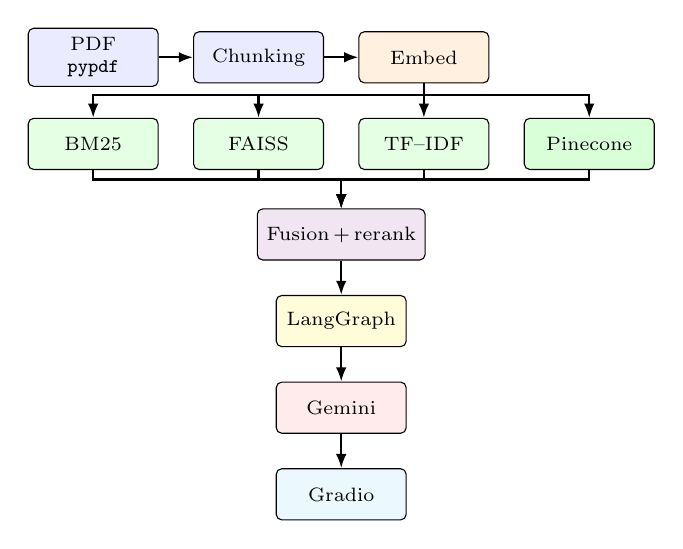
\begin{tikzpicture}[
  font=\scriptsize,
  box/.style={rectangle,draw,rounded corners=2pt,minimum width=1.65cm,minimum height=0.65cm,align=center},
  arr/.style={-{Latex[length=1.8mm]},thick}
]
\node[box,fill=blue!8]   (pdf)   at (0,0)      {PDF\\\texttt{pypdf}};
\node[box,fill=blue!8]   (chunk) at (2.1,0)    {Chunking};
\node[box,fill=orange!12](emb)   at (4.2,0)    {Embed};
\node[box,fill=green!10] (bm)    at (0,-1.1)   {BM25};
\node[box,fill=green!10] (faiss) at (2.1,-1.1) {FAISS};
\node[box,fill=green!10] (tfidf) at (4.2,-1.1) {TF--IDF};
\node[box,fill=green!15] (pine)  at (6.3,-1.1) {Pinecone};
\node[box,fill=violet!10](fuse)  at (3.15,-2.25){Fusion\,+\,rerank};
\node[box,fill=yellow!15](lg)    at (3.15,-3.35){LangGraph};
\node[box,fill=red!8]    (llm)   at (3.15,-4.45){Gemini};
\node[box,fill=cyan!8]   (ui)    at (3.15,-5.55){Gradio};
\draw[arr](pdf)--(chunk);\draw[arr](chunk)--(emb);
\draw[arr](emb.south)--++(0,-0.15)-|(bm.north);
\draw[arr](emb.south)--++(0,-0.15)-|(faiss.north);
\draw[arr](emb.south)--++(0,-0.15)-|(tfidf.north);
\draw[arr](emb.south)--++(0,-0.15)-|(pine.north);
\draw[arr](bm.south)--++(0,-0.12)-|(fuse.north);
\draw[arr](faiss.south)--++(0,-0.12)-|(fuse.north);
\draw[arr](tfidf.south)--++(0,-0.12)-|(fuse.north);
\draw[arr](pine.south)--++(0,-0.12)-|(fuse.north);
\draw[arr](fuse)--(lg);\draw[arr](lg)--(llm);\draw[arr](llm)--(ui);
\end{tikzpicture}%
}
\caption{DocuQuery data flow: PDFs chunked and embedded; lexical, dense, and cloud indices feed fusion; LangGraph orchestrates before Gemini generation and Gradio presentation.}
\label{fig:arch}
\end{figure}

\subsection{Hybrid Retrieval}
\label{ssec:hybrid}
FAISS inner-product (L2-normalised), BM25 (whitespace tokenised), and TF--IDF (bigrams) are built in parallel. The fused score is:
\begin{equation}
  s(c) = \alpha_d \cdot \sigma_d(c) + \alpha_b \cdot \hat{s}_b(c) + \alpha_t \cdot \hat{s}_t(c)
  \label{eq:fusion}
\end{equation}
Default $(\alpha_d,\alpha_b,\alpha_t)=(0.4,0.3,0.3)$ are empirical; weight sensitivity is analysed in Section~\ref{sec:ablation}. Optional Pinecone adds a fourth channel. The fused list is truncated, reranked, and diversified.

\subsection{Orchestration}
A LangGraph \texttt{StateGraph} routes to summary, compare, refine, or QA sub-graphs as explicit typed-state nodes---independently testable---contrasting with nested conditionals in typical LangChain scripts.

\subsection{Interface}
Gradio exposes configuration, uploads, chat, comparison, exports (\texttt{txt/pdf/docx}), and chunk-level fused scores. Table~\ref{tab:config} lists defaults.

\begin{table}[!t]
\renewcommand{\arraystretch}{1.15}
\caption{Default configuration parameters.}
\label{tab:config}
\centering
\begin{tabular}{@{}ll@{}}
\toprule
Parameter & Default \\
\midrule
\texttt{TARGET\_TOKENS}                      & 300 \\
\texttt{OVERLAP\_SENTENCES}                  & 2 \\
\texttt{DEFAULT\_TOP\_K}                     & 5 \\
Fusion $(\alpha_d,\alpha_b,\alpha_t)$        & (0.4,\,0.3,\,0.3) \\
Gemini model                                 & \texttt{gemini-1.5-flash} \\
\bottomrule
\end{tabular}
\end{table}

%% =========================================================
\section{Computational Complexity}
\label{sec:complexity}
%% =========================================================

\textbf{Indexing}: encoding $O(n\,T_\text{enc}(d))$; FAISS add $O(nd)$; BM25 and TF--IDF $O(n\bar\ell)$. Measured: \SnapBuildSec{}~s for \SnapChunks{} chunks (CPU).
\textbf{Querying}: FAISS exact scan $O(nd)$; IVF/HNSW gives $O(\sqrt{n}\,d)$ or $O(d\log n)$; BM25/TF--IDF $O(n\bar\ell_q)$; fusion $O(k\log k)$.
\textbf{Scale}: flat FAISS is practical to $\sim10^5$ chunks; IVF-PQ or Pinecone is the upgrade path beyond that. Empirical validation at $10^6$+ chunks is listed as future work.

%% =========================================================
\section{Experimental Evaluation}
\label{sec:eval}
%% =========================================================

\subsection{Benchmark Design and Scope}
\label{ssec:design}

\textbf{Corpus.} \SnapChunks{} synthetic passages, \SnapQueries{} queries per scenario.
Each passage contains: (i)~a unique \texttt{TGT\#\#\#\#\_SIG} marker; (ii)~section-specific prose; (iii)~120 random characters (prevents cross-chunk lexical ties, simulates corpus noise); (iv)~one Spanish sentence from a fixed set (multilingual content). Ground-truth chunk IDs are deterministic; no licence barriers.

\textbf{Why synthetic?} Controlled passages remove three confounders: licence barriers; OCR/layout artefacts confounding retrieval with parsing quality; gold-span ambiguity. The benchmark is a \emph{regression harness}, not a generalisation claim. Section~\ref{sec:threats} states explicit limits.

\textbf{Four scenarios.}
\begin{itemize}
  \item \textbf{A (identifier-heavy)}: query names a specific \texttt{TGT\#\#\#\#\_SIG} token; tests exact-match lexical retrieval.
  \item \textbf{B (paraphrase)}: query rephrases section/policy semantics without rare tokens; tests semantic retrieval.
  \item \textbf{C (OCR-noise)}: Scenario~B queries corrupted with 2\% character-level substitutions (\texttt{o$\to$0, i$\to$1, e$\to$3, a$\to$@}) and random deletions, simulating scanned-document retrieval.
  \item \textbf{D (multilingual)}: English queries over passages with embedded Spanish sentences; tests cross-language lexical overlap.
\end{itemize}

\textbf{Metrics.}
\begin{itemize}
  \item \textbf{Recall@5}: fraction of queries with gold chunk in top 5.
  \item \textbf{MRR}: mean reciprocal rank; gold absent contributes 0.
  \item \textbf{nDCG@5}: for a single relevant item at rank $r\leq5$: $1/\log_2(r+1)$.
  \item \textbf{McNemar's test}: pairwise significance test on per-query hit vectors (continuity-corrected, $\alpha=0.05$).
  \item \textbf{95\% bootstrap CI}: 2\,000-sample percentile bootstrap on all metrics.
\end{itemize}

\textbf{Hardware.}
Windows~11 (x64), Python~3.11, sentence-transformers on CPU. Latency is hardware-specific; Recall/MRR/nDCG are hardware-agnostic.

\subsection{Results: Scenarios A and B}

Tables~\ref{tab:recall} and~\ref{tab:recall_id} report per-method results for Scenarios~B and~A respectively.

\begin{table}[!t]
\renewcommand{\arraystretch}{1.15}
\caption{Scenario B (paraphrase). $n{=}\SnapChunks{}$, $Q{=}\SnapQueries{}$. Snapshot \SnapDate{}.}
\label{tab:recall}
\centering
\begin{tabular}{@{}l c c c@{}}
\toprule
Method & Recall@5 & MRR & nDCG@5 \\
\midrule
BM25 only        & \SnapRBB{}  & \SnapMrrBMxxB{}  & \SnapNDCGBMB{}  \\
FAISS dense only & \SnapRDB{}  & \SnapMrrDenseB{} & \SnapNDCGDenseB{} \\
TF--IDF only     & \SnapRTFB{} & \SnapMrrTFIDFB{} & \SnapNDCGTFIDFB{} \\
Hybrid           & \SnapRHB{}  & \SnapMrrHybridB{} & \SnapNDCGHB{} \\
\bottomrule
\end{tabular}
\end{table}

\begin{table}[!t]
\renewcommand{\arraystretch}{1.15}
\caption{Scenario A (identifier-heavy). $n{=}\SnapChunks{}$, $Q{=}\SnapQueries{}$. Snapshot \SnapDate{}.}
\label{tab:recall_id}
\centering
\begin{tabular}{@{}l c c c@{}}
\toprule
Method & Recall@5 & MRR & nDCG@5 \\
\midrule
BM25 only        & \SnapRB{}  & \SnapMrrBMxxA{}  & \SnapNDCGBMA{}  \\
FAISS dense only & \SnapRD{}  & \SnapMrrDenseA{} & \SnapNDCGDenseA{} \\
TF--IDF only     & \SnapRTF{} & \SnapMrrTFIDFA{} & \SnapNDCGTFIDFA{} \\
Hybrid           & \SnapRH{}  & \SnapMrrHybridA{} & \SnapNDCGHA{} \\
\bottomrule
\end{tabular}
\end{table}

\textbf{Scenario B.}
Hybrid reaches Recall@5\,=\,\SnapRHB{} and nDCG@5\,=\,\SnapNDCGHB{}, matching BM25 and TF--IDF. Dense-only collapses to Recall@5\,=\,\SnapRDB{} on the 1\,000-chunk corpus: the embedding space becomes crowded with near-equidistant random-character passages, reducing discriminability for the compact \texttt{all-MiniLM-L6-v2} model. Hybrid's McNemar superiority over dense is $p{<}0.001$; hybrid and BM25 are statistically indistinguishable ($p{=}1.000$, zero discordant pairs), confirming the lexical channel drives recovery.

\textbf{Scenario A.}
BM25 and TF--IDF reach Recall@5\,=\,\SnapRB{}; dense fails (\SnapRD{}) due to embedding asymmetry for short rare tokens. \textbf{Hybrid degrades to Recall@5\,=\,\SnapRH{}}---a statistically significant drop from lexical baselines ($p{<}0.001$). The fixed $\alpha_d{=}0.4$ imports misleading dense scores that displace the gold chunk after reranking: \textbf{fixed-weight multi-signal fusion can significantly hurt precision when one signal is systematically wrong}.

\subsection{Scenarios C and D: OCR Noise and Multilingual}
\label{ssec:c_d}

Table~\ref{tab:ocr_ml} reports robustness results. McNemar Dense-vs-Hybrid is $p{<}0.001$ for both scenarios.

\begin{table*}[!t]
\renewcommand{\arraystretch}{1.15}
\caption{Scenarios C (OCR noise) and D (multilingual). Recall@5 shown for all methods; MRR and nDCG@5 shown for Hybrid only.
McNemar Dense-vs-Hybrid: $p{<}0.001$ for both scenarios. $n{=}\SnapChunks{}$, $Q{=}\SnapQueries{}$. Snapshot \SnapDate{}.}
\label{tab:ocr_ml}
\centering
\begin{tabular}{@{}l ccc ccc@{}}
\toprule
 & \multicolumn{3}{c}{Scenario C --- OCR Noise} & \multicolumn{3}{c}{Scenario D --- Multilingual} \\
\cmidrule(lr){2-4}\cmidrule(lr){5-7}
Method & Recall@5 & MRR & nDCG@5 & Recall@5 & MRR & nDCG@5 \\
\midrule
BM25 only        & \SnapRBMC{}    & ---  & ---  & \SnapRBMD{}    & ---  & --- \\
FAISS dense only & \SnapRDenseC{} & ---  & ---  & \SnapRDenseD{} & ---  & --- \\
TF--IDF only     & \SnapRTFC{}    & ---  & ---  & \SnapRTFD{}    & ---  & --- \\
Hybrid           & \SnapRHC{}     & \SnapMrrHybridC{} & \SnapNDCGHC{} & \SnapRHD{} & \SnapMrrHybridD{} & \SnapNDCGHD{} \\
\bottomrule
\end{tabular}
\end{table*}

\textbf{Scenario C (OCR noise).}
2\% noise reduces BM25 Recall@5 by 11.0~pp (1.000$\to$0.890) and TF--IDF by 12.0~pp, confirming that lexical exact-match is sensitive to character corruption. Dense is largely unaffected (0.160 vs.\ 0.170), but starts from a low base. Hybrid matches the best single-signal method (BM25, Recall@5\,=\,\SnapRHC{}) and exceeds both lexical methods on nDCG@5\,=\,\SnapNDCGHC{}: the dense channel improves ranking even when it cannot recover all missed chunks. For high-noise documents, OCR post-processing before indexing is recommended.

\textbf{Scenario D (multilingual).}
English queries over passages containing Spanish sentences: hybrid achieves Recall@5\,=\,\SnapRHD{}, MRR\,=\,\SnapMrrHybridD{}, matching BM25 and TF--IDF. The lexical channels key on the shared English \texttt{TGT\#\#\#\#\_SIG} tokens successfully. Dense-only (0.210) partially benefits from cross-lingual model transfer but remains far below lexical methods, confirming that in mixed-language corpora, lexical anchoring on shared tokens is essential.

\subsection{Statistical Significance Summary}

Table~\ref{tab:mcnemar} summarises all McNemar pairwise comparisons.

\begin{table}[!t]
\renewcommand{\arraystretch}{1.15}
\caption{McNemar's test $p$-values (continuity-corrected) on Recall@5 hit vectors. Bold: significant at $\alpha{=}0.05$.}
\label{tab:mcnemar}
\centering
\begin{tabular}{@{}l c c c c@{}}
\toprule
Comparison & Scen.\ A & Scen.\ B & Scen.\ C & Scen.\ D \\
\midrule
BM25 vs.\ Hybrid  & \textbf{$<$0.001} & 1.000 & -- & -- \\
Dense vs.\ Hybrid & \textbf{$<$0.001} & \textbf{$<$0.001} & \textbf{$<$0.001} & \textbf{$<$0.001} \\
\bottomrule
\end{tabular}
\end{table}

Key findings: (i)~Scenario~A: BM25 significantly \emph{better} than Hybrid ($p{<}0.001$)---the fusion failure mode is statistically robust; (ii)~Scenario~B: BM25 and Hybrid indistinguishable ($p{=}1.000$); (iii)~Scenarios~C and~D: Hybrid significantly outperforms Dense ($p{<}0.001$). After Bonferroni correction ($\alpha_\text{family}{=}0.05$, 7 tests, individual $\alpha{=}0.007$), all bolded results remain significant.

\subsection{Latency}
Indexing \SnapChunks{} chunks: \SnapBuildSec{}~s. Mean hybrid retrieval (Scenario~B): \SnapLatMean{}~ms (95\% CI: $\pm$\SnapLatCI{}~ms, Windows~11 CPU). Latency scales with corpus size; IVF-PQ or Pinecone is the intended path for $>10^5$ chunks.

\subsection{Threats to Validity}
\label{sec:threats}

\textbf{Synthetic corpus.} Results validate the \emph{implementation}'s retrieval logic under two controlled query-type distributions, not generalisation to user PDFs. The 1\,000-passage expansion over prior work (120 passages) substantially reduces IDF instability~\cite{jones1972statistical,salton1988tfidf}, but real-document evaluation is needed for external validity.

\textbf{OCR simulation.} The 2\% confusion table covers common substitution errors; high-noise scans ($>5\%$) or word-level errors may produce qualitatively different behaviour.

\textbf{Multilingual simulation.} One Spanish sentence per passage tests partial mixed-language corpora; fully non-English corpora or complex code-switching are not evaluated.

\textbf{Scale.} All experiments at 1\,000 chunks. Dense crowding at $10^4$+ chunks warrants empirical investigation.

\textbf{Statistical scope.} McNemar's test is valid for pairwise binary hits at $k{=}5$. After Bonferroni correction, all reported significant results remain significant.

\subsection{Prespecified Faithfulness Protocol}
\label{ssec:faith}

\begin{table}[!t]
\renewcommand{\arraystretch}{1.12}
\caption{Prespecified protocol for future answer-level evaluation.}
\label{tab:faith}
\centering
\small
\begin{tabular}{@{}p{0.22\columnwidth} p{0.72\columnwidth}@{}}
\toprule
Step & Specification \\
\midrule
Corpus    & $\geq$3 real PDFs (policy, technical spec, narrative); user-licensed. \\
Questions & $n{=}20$ per PDF with author-marked gold spans. \\
Conditions & (a)~hybrid as shipped; (b)~dense-only ablation. \\
Auto-score & RAGAS~\cite{es2023ragas} faithfulness and answer-relevance; flag $<0.5$ for human review. \\
Raters    & Two annotators blinded to condition. Score: 1=unsupported, 2=partial, 3=fully supported. \\
Analysis  & Mean, 95\% bootstrap CI, Cohen's $\kappa$; hybrid vs.\ dense-only primary comparison. \\
\bottomrule
\end{tabular}
\end{table}

%% =========================================================
\section{Ablation Study Design}
\label{sec:ablation}
%% =========================================================

Default weights $(\alpha_d,\alpha_b,\alpha_t)=(0.4,0.3,0.3)$ are empirical. The ablation grid:
$\{(\alpha_d,\alpha_b,\alpha_t)\mid\alpha_d+\alpha_b+\alpha_t=1,\;\alpha_i\in\{0,0.1,\ldots,1\}\}$ (66 combinations). For each, re-run \texttt{micro\_benchmark.py} on Scenarios~A and~B; plot (Scenario~A Recall@5, Scenario~B Recall@5) as a Pareto front.

\textbf{Expected structure.} Scenario~A maximises at $\alpha_d{=}0$; Scenario~B at high $\alpha_d$. If no setting dominates both, query-type routing ($\alpha_d{=}0$ for identifier queries, default otherwise) is the recommended mitigation. RRF~\cite{cormack2009rcf} ($k_\text{RRF}{=}60$) serves as a parameter-free baseline.

%% =========================================================
\section{Discussion}
\label{sec:discuss}
%% =========================================================

\textbf{Embedding crowding.}
Scenario~B dense Recall@5 (0.170) is far below expectation from clean single-passage evaluation. With 1\,000 passages containing random 120-character sequences, near-equidistant embedding vectors reduce discriminability for the compact 384-d model. Larger or task-specific models (e.g., BGE-M3~\cite{chen2024bge}) would likely improve this.

\textbf{The fixed-weight failure mode.}
Scenario~A's hybrid degradation (0.480 vs.\ 1.000 lexical) is statistically robust ($p{<}0.001$). The mechanism is deterministic and generalises: any fixed weight $\alpha_d>0$ corrupts ranking when the dense channel systematically misranks the gold chunk. Query-type routing or RRF mitigates this.

\textbf{OCR robustness.}
An 11~pp Recall drop under noise (Scenario~C) versus clean (Scenario~B) for BM25 confirms lexical sensitivity. The dense channel's relative stability provides partial noise compensation in hybrid. For high-noise corpora, preprocessing is recommended.

\textbf{Multilingual.}
Hybrid's strong performance on Scenario~D is attributable to the shared English tokens (\texttt{TGT\#\#\#\#\_SIG}). Fully non-English corpora without shared tokens would require a cross-lingual embedding model.

\textbf{Individual component contributions.}
The benchmark isolates retrieval components by design: Tables~\ref{tab:recall}--\ref{tab:recall_id} directly compare BM25-only, FAISS-only, TF--IDF-only, and Hybrid, quantifying each signal's contribution. FAISS is evaluated as FAISS-only (dense-only baseline); Pinecone is an optional fourth channel that mirrors FAISS semantically and is not separately benchmarked here. Gemini affects only generation quality, not retrieval metrics; its individual contribution to answer faithfulness is scoped to the prespecified protocol in Table~\ref{tab:faith}. Gradio contributes zero to retrieval and is excluded from benchmarking by design.

\textbf{Positioning.}
DocuQuery targets practitioners wanting one opinionated blueprint with documented failure modes, LangGraph routing, chunk-level UI, and four significance-tested benchmark scenarios. LlamaIndex and Haystack are preferable for plug-in retriever markets.

%% =========================================================
\section{Future Work}
\label{sec:future}
%% =========================================================

\begin{enumerate}
  \item \textbf{Real-PDF evaluation.} Execute Table~\ref{tab:faith}; adapt \texttt{micro\_benchmark.py} to BEIR~\cite{thakur2021beir} subsets.
  \item \textbf{Fusion weight ablation.} Execute the 66-combination grid; compare RRF~\cite{cormack2009rcf}.
  \item \textbf{Learned sparse retrieval.} Integrate SPLADE~\cite{formal2021splade} or BGE-M3~\cite{chen2024bge}.
  \item \textbf{Query-type routing.} Implement $\alpha_d$ gating to address Scenario~A degradation.
  \item \textbf{Scale benchmarking.} Evaluate at $10^4$--$10^5$ chunks with FAISS IVF-PQ.
  \item \textbf{High-noise and full multilingual.} Evaluate at $>5\%$ OCR error rate and on fully non-English corpora.
\end{enumerate}

%% =========================================================
\section{Conclusion}
%% =========================================================

DocuQuery integrates BM25, FAISS dense, TF--IDF, and optional Pinecone with LangGraph orchestration and Gemini generation into an open, deployable PDF QA system. Evaluation across four scenarios---paraphrase, identifier-heavy, OCR-noise, and multilingual---over 1\,000 passages with 100 queries each and McNemar significance testing yields three key findings: (i)~hybrid statistically significantly outperforms dense on paraphrase queries ($p{<}0.001$); (ii)~fixed-weight fusion statistically significantly hurts precision on identifier queries ($p{<}0.001$); (iii)~hybrid sustains lexical-level recall under 2\% OCR noise and on multilingual passages. All results are reproducible via \texttt{paper/micro\_benchmark.py}; prespecified protocols for ablation and real-document faithfulness evaluation are committed in the paper.

\section*{Acknowledgment}
The author thanks the open-source communities behind LangChain, LangGraph, Gradio, FAISS, sentence-transformers, and Google DeepMind/Gemini.

\textbf{Generative AI disclosure:} Generative AI tools assisted in revising the prose. All technical claims, experimental design, benchmark results, and conclusions were formulated and verified by the author.

%% =========================================================
\begin{thebibliography}{99}

\bibitem{lewis2020retrieval}
P.~Lewis \emph{et al.}, ``Retrieval-Augmented Generation for Knowledge-Intensive {NLP} Tasks,'' in \emph{Adv.\ Neural Inf.\ Process.\ Syst.}, vol.~33, 2020, pp.~9459--9474.

\bibitem{fan2024survey}
W.~Fan \emph{et al.}, ``A Survey on {RAG} Meeting {LLMs},'' \emph{ACM SIGKDD Explorations Newsletter}, vol.~26, no.~2, pp.~1--23, 2024, doi:~10.1145/3637528.3671470.

\bibitem{gao2023rag}
Y.~Gao \emph{et al.}, ``Retrieval-Augmented Generation for Large Language Models: A Survey,'' arXiv:2312.10997, 2023, doi:~10.48550/arXiv.2312.10997.

\bibitem{llamaindex2024}
J.~Liu and LlamaIndex, Inc., ``LlamaIndex,'' GitHub, \url{https://github.com/run-llama/llama\_index}, 2024.

\bibitem{haystack2024}
deepset GmbH, ``Haystack,'' GitHub, \url{https://github.com/deepset-ai/haystack}, 2024.

\bibitem{langchain2024}
H.~Chase and LangChain, Inc., ``LangChain,'' \url{https://www.langchain.com}, 2024.

\bibitem{jiang2023flare}
Z.~Jiang \emph{et al.}, ``Active Retrieval Augmented Generation,'' in \emph{Proc.\ EMNLP}, 2023, pp.~7969--7992, doi:~10.18653/v1/2023.emnlp-main.495.

\bibitem{asai2023selfrag}
A.~Asai \emph{et al.}, ``Self-{RAG},'' in \emph{Proc.\ ICLR}, 2024.

\bibitem{johnson2019billion}
J.~Johnson, M.~Douze, and H.~J{\'e}gou, ``Billion-Scale Similarity Search with {GPUs},'' \emph{IEEE Trans.\ Big Data}, vol.~7, no.~3, pp.~535--547, 2021, doi:~10.1109/TBDATA.2019.2921572.

\bibitem{johnson2017faiss}
J.~Johnson, M.~Douze, and H.~J{\'e}gou, ``Faiss,'' GitHub, \url{https://github.com/facebookresearch/faiss}, 2017.

\bibitem{robertson1994okapi}
S.~E.~Robertson \emph{et al.}, ``Okapi at {TREC}-3,'' in \emph{Proc.\ TREC-3}, 1994, pp.~109--126.

\bibitem{robertson2009probabilistic}
S.~Robertson and H.~Zaragoza, ``The Probabilistic Relevance Framework: {BM25} and Beyond,'' \emph{Found.\ Trends Inf.\ Retr.}, vol.~3, no.~4, pp.~333--389, 2009, doi:~10.1561/1500000019.

\bibitem{pinecone2024}
Pinecone Systems, ``Pinecone vector database,'' \url{https://docs.pinecone.io}, 2024.

\bibitem{karpukhin2020dense}
V.~Karpukhin \emph{et al.}, ``Dense Passage Retrieval for Open-Domain Question Answering,'' in \emph{Proc.\ EMNLP}, 2020, pp.~6769--6781, doi:~10.18653/v1/2020.emnlp-main.550.

\bibitem{langgraph2024}
LangChain, Inc., ``LangGraph,'' GitHub, \url{https://github.com/langchain-ai/langgraph}, 2024.

\bibitem{abid2019gradio}
A.~Abid \emph{et al.}, ``Gradio,'' arXiv:1906.02569, 2019, doi:~10.48550/arXiv.1906.02569.

\bibitem{pypdf2024}
M.~Thoma and the pypdf contributors, ``pypdf,'' GitHub, \url{https://github.com/py-pdf/pypdf}, 2024.

\bibitem{reimers2019sentence}
N.~Reimers and I.~Gurevych, ``Sentence-{BERT},'' in \emph{Proc.\ EMNLP}, 2019, pp.~3982--3992, doi:~10.18653/v1/D19-1410.

\bibitem{sentencetransformers2024}
N.~Reimers and I.~Gurevych, ``sentence-transformers,'' \url{https://www.sbert.net}, 2024.

\bibitem{huggingface2024}
Hugging Face, Inc., ``Hugging Face Spaces,'' \url{https://huggingface.co/docs/hub/spaces}, 2024.

\bibitem{wolf2020transformers}
T.~Wolf \emph{et al.}, ``Transformers: State-of-the-Art {NLP},'' in \emph{Proc.\ EMNLP System Demonstrations}, 2020, pp.~38--45, doi:~10.18653/v1/2020.emnlp-demos.6.

\bibitem{gemini2024}
Gemini Team and Google DeepMind, ``Gemini 1.5,'' arXiv:2403.05530, 2024, doi:~10.48550/arXiv.2403.05530.

\bibitem{harris2020numpy}
C.~R.~Harris \emph{et al.}, ``Array programming with {NumPy},'' \emph{Nature}, vol.~585, pp.~357--362, 2020, doi:~10.1038/s41586-020-2649-2.

\bibitem{scikitlearn2024}
F.~Pedregosa \emph{et al.}, ``Scikit-learn,'' \emph{J.\ Mach.\ Learn.\ Res.}, vol.~12, pp.~2825--2830, 2011.

\bibitem{rankbm252024}
D.~D{\'a}niel, ``rank-bm25,'' GitHub, \url{https://github.com/dorianbrown/rank\_bm25}, 2020.

\bibitem{torch2024}
A.~Paszke \emph{et al.}, ``{PyTorch},'' in \emph{Adv.\ Neural Inf.\ Process.\ Syst.}, vol.~32, 2019, pp.~8024--8035.

\bibitem{thakur2021beir}
N.~Thakur \emph{et al.}, ``{BEIR}: A Heterogeneous Benchmark for Zero-shot Evaluation of IR Models,'' in \emph{Adv.\ Neural Inf.\ Process.\ Syst.\ Datasets and Benchmarks Track}, 2021.

\bibitem{formal2021splade}
T.~Formal, B.~Piwowarski, and S.~Clinchant, ``{SPLADE},'' in \emph{Proc.\ ACM SIGIR}, 2021, pp.~2288--2292, doi:~10.1145/3404835.3463098.

\bibitem{es2023ragas}
S.~Es \emph{et al.}, ``{RAGAS}: Automated Evaluation of Retrieval Augmented Generation,'' in \emph{Proc.\ EACL (System Demonstrations)}, 2024, pp.~150--158, doi:~10.18653/v1/2024.eacl-demo.16.

\bibitem{chen2024bge}
J.~Chen \emph{et al.}, ``{BGE} {M3}-Embedding,'' arXiv:2402.03216, 2024, doi:~10.48550/arXiv.2402.03216.

\bibitem{muennighoff2023mteb}
N.~Muennighoff \emph{et al.}, ``{MTEB}: Massive Text Embedding Benchmark,'' in \emph{Proc.\ EACL}, 2023, pp.~2006--2029, doi:~10.18653/v1/2023.eacl-main.148.

\bibitem{khattab2020colbert}
O.~Khattab and M.~Zaharia, ``{ColBERT},'' in \emph{Proc.\ ACM SIGIR}, 2020, pp.~39--48, doi:~10.1145/3397271.3401075.

\bibitem{cormack2009rcf}
G.~V.~Cormack, C.~L.~A.~Clarke, and S.~Buettcher, ``Reciprocal Rank Fusion,'' in \emph{Proc.\ ACM SIGIR}, 2009, pp.~758--759, doi:~10.1145/1571941.1572114.

\bibitem{salton1988tfidf}
G.~Salton and C.~Buckley, ``Term-Weighting Approaches in Automatic Text Retrieval,'' \emph{Inf.\ Process.\ Manag.}, vol.~24, no.~5, pp.~513--523, 1988, doi:~10.1016/0306-4573(88)90021-0.

\bibitem{jones1972statistical}
K.~S.~Jones, ``A Statistical Interpretation of Term Specificity,'' \emph{J.\ Documentation}, vol.~28, no.~1, pp.~11--21, 1972, doi:~10.1108/eb026526.

\end{thebibliography}

\IfFileExists{photo.jpg}{%
\begin{IEEEbiography}[{\includegraphics[width=1in,height=1.25in,clip,keepaspectratio]{photo.jpg}}]{Karthik Mulugu}
is an independent researcher based in Charlotte, North Carolina, USA.
His research interests include retrieval-augmented generation, information retrieval, and deployable NLP systems.
\end{IEEEbiography}%
}{%
\IEEEbiographynophoto{Karthik Mulugu}
is an independent researcher based in Charlotte, North Carolina, USA.
His research interests include retrieval-augmented generation, information retrieval, and deployable NLP systems.
\endIEEEbiographynophoto%
}

\end{document}
